%%%%%%%%%%%%%%%%%%%%%%%%%%%%%%%%%%%%%%%%%%%%%%%%%%%%%%%%%%%%%%%%%%%%%%%%%%
% File: Lecture_1.tex
% Authors: James Kress
% Date: February 1, 2014
% Description: 
%%%%%%%%%%%%%%%%%%%%%%%%%%%%%%%%%%%%%%%%%%%%%%%%%%%%%%%%%%%%%%%%%%%%%%%%%%

%<<<<<<<<<<<<<<<<<<<<<<<<<<<<<<<<<<<<<<<<<<<<<<<<<<<<<<<<<<<<<<<<<<<<<<<<<<<<<%
% Document package information
%>>>>>>>>>>>>>>>>>>>>>>>>>>>>>>>>>>>>>>>>>>>>>>>>>>>>>>>>>>>>>>>>>>>>>>>>>>>>>%
\documentclass[xcolor=dvipsnames]{beamer} 
%%%%%%%%%%%%%%%%%%%%%%%%%%%%%%%%%%%%%%%%%%%%%%%%%%%%%%%%%%%%%%%%%%%%%%%%%%
% File: _TeXdefs.tex
% Author: James Kress
% Date: January 25, 2014
% Description: A tex file containing the \usepackage declarations, and
%			   other document critial style settings.
%%%%%%%%%%%%%%%%%%%%%%%%%%%%%%%%%%%%%%%%%%%%%%%%%%%%%%%%%%%%%%%%%%%%%%%%%%

%-----------Package imports
\usepackage{graphicx}
\usepackage{pgfpages}
\usepackage{tikz}
\usepackage{latexsym}
\usepackage{verbatim}
%//////////END package imports


%----------Style elements
\useoutertheme{infolines} 
\usetheme{Frankfurt} 
\usepackage{../theme/beamercolorthemeoregon}
\setbeamertemplate{sections/subsections in toc}[default]
\setbeamertemplate{footline}
{
\leavevmode%
  \hbox{%
  \begin{beamercolorbox}[wd=.3\paperwidth,ht=2.25ex,dp=.75ex,center]{institute in head/foot}%
    \usebeamerfont{institute in head/foot}\insertshortinstitute
  \end{beamercolorbox}%
    \begin{beamercolorbox}[wd=.4\paperwidth,ht=2.25ex,dp=.75ex,center]{title in head/foot}%
      \usebeamerfont{title in head/foot}\insertshorttitle
    \end{beamercolorbox}%
  \begin{beamercolorbox}[wd=.3\paperwidth,ht=2.25ex,dp=.75ex,center]{date in head/foot}%
    \usebeamerfont{date in head/foot}\insertshortdate\hspace*{3em}
    \insertframenumber{} / \inserttotalframenumber\hspace*{1ex}
  \end{beamercolorbox}}%
  \vskip0pt%
}
%/////////END style elements


%---------Command Declarations
\DeclareGraphicsExtensions{.pdf, .jpeg, .png, .jpg}
\graphicspath{ {../images/} }
\newcommand{\className}{\text{CIS 410/510} \\ \text{Parallel Computing}}
\newcommand{\departmentName}{\textit{Department of Computer and 
									Information Science \\ University of Oregon}}
%/////////END command declarations


%---------Setup pdf properties
\hypersetup{
	pdfusetitle=true,
    bookmarks=true,         	% show bookmarks bar?
    unicode=false,          	% non-Latin characters in Acrobat’s bookmarks
    pdftoolbar=true,        	% show Acrobat’s toolbar?
    pdfmenubar=true,        	% show Acrobat’s menu?
    pdffitwindow=false,     	% window fit to page when opened
    pdfstartview={Fit},   		% fits the width of the page to the window    
    pdfauthor={},     % author
    pdfsubject={Parallel Programming},   	% subject of the document
    pdfcreator={},   			% creator of the document
    pdfproducer={}, 			% producer of the document
    pdfkeywords={University of Oregon, parallel programming}, 
    pdfnewwindow=true,      	% links in new window
    colorlinks=true,       		% false: boxed links; true: colored links
    linkcolor=white,          	% color of internal links
    hidelinks,
    citecolor=green,        	% color of links to bibliography
    filecolor=magenta,      	% color of file links
    urlcolor=cyan,           	% color of external links
    linktoc=page,
    pageanchor = true
}
%//////////END setup pdf properties


%END ALL


\usepackage{listings}
%<<<<<<<<<<<<<<<<<<<<<<<<<<<<<<<<<<<<<<<<<<<<<<<<<<<<<<<<<<<<<<<<<<<<<<<<<<<<<%
% END Document package information
%>>>>>>>>>>>>>>>>>>>>>>>>>>>>>>>>>>>>>>>>>>>>>>>>>>>>>>>>>>>>>>>>>>>>>>>>>>>>>%

%=============================================================================%
% Begining: Title Page Material
%=============================================================================%
\begin{document}
	\title[Matrix Multiplication]{Matrix Multiplication}
	\author[]{\className}
	\institute[\className]{\departmentName}
	\date{} 

	\titlegraphic{\centering 
		$\vcenter{\hbox{
\includegraphics[height=.31in,width=2.0in]{oregonLogo}}}$
	}

	\begin{frame}
		\maketitle
	\end{frame}
	
	%--- Next Frame ---%

	\begin{frame}{Definition}
		\begin{equation*}
			A =
			\begin{bmatrix}
				A_{11} & A_{12} & \ldots & A_{1p} \\
				A_{21} & A_{22} & \ldots & A_{2p} \\
				\vdots & \vdots & \ddots & \vdots \\
				A_{m1} & A_{m2} & \ldots & A_{mp}
			\end{bmatrix}, 
			B =
			\begin{bmatrix}
				B_{11} & B_{12} & \ldots & B_{1n} \\
				B_{21} & B_{22} & \ldots & B_{2n} \\
				\vdots & \vdots & \ddots & \vdots \\
				A_{p1} & B_{p2} & \ldots & B_{pn}
			\end{bmatrix}
		\end{equation*}
		\begin{equation*}
			C = A \times B = 
			\begin{bmatrix}
				C_{11} & C_{12} & \ldots & C_{1n} \\
				C_{21} & C_{22} & \ldots & C_{2n} \\
				\vdots & \vdots & \ddots & \vdots \\
				C_{m1} & C_{m2} & \ldots & C_{mn}
			\end{bmatrix}
		\end{equation*}
		\begin{equation*}
			C_{ij} = \sum_{k=1}^p{A_{ik}B_{kj}}
		\end{equation*}
	\end{frame}

	%--- Next Frame ---%

	\begin{frame}{Definition}
		\begin{center}
		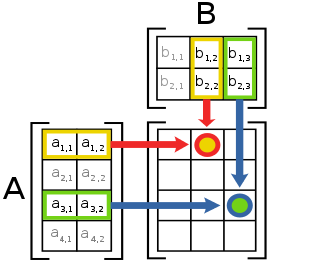
\includegraphics[scale=0.5]{images/multip}
		\footnote{Picture from wikipedia}
		\end{center}
	\end{frame}

	%--- Next Frame ---%

	\defverbatim[colored]\lstnaive{%
	\begin{lstlisting}[tabsize=8,basicstyle=\ttfamily]
	for (i=0; i<M; i++) {
	    for (j=0; j<N; j++) {
		C[i][j] = 0;
		for (k=0; k<P; k++) {
		    C[i][j] += A[i][k] * B[k][j];
		}
	    }
	}
	\end{lstlisting}
	}

	\begin{frame}{Naive implementation}
		\lstnaive
	\end{frame}

	%--- Next Frame ---%
	\defverbatim[colored]\lsttmp{%
	\begin{lstlisting}[tabsize=8,basicstyle=\ttfamily]
	double tmp = 0.0;
	for (k=0; k<P; i++) {
	    tmp += A[i][k] * B[k][j];
	}
	C[i][j] = tmp;
	\end{lstlisting}
	}

	\begin{frame}{Warm up}
		\begin{itemize}
			\item A serial implementation is provided
			\item \underline{FIXME: need unified method to get sample code}
			\item Compile and run

			% 1. inner loop, use a temp variable instead of C[i][j] directly
			% 2. loop interchange: swith the 2nd and 3rd loop
			% 3. 1 and 2 are not compatible
			\item Discussion: What's the problem with this program?

			\item Fix it, try again
		\end{itemize}
	\end{frame}
	
	%--- Next Frame ---%
	
	\begin{frame}{OpenMP Quick Review}
		\begin{itemize}
			\item \#pragma omp parallel
			\item \#pragma omp for
			\item \#pragma omp parallel for
			\item int omp\_set\_num\_threads();
			\item int omp\_get\_num\_threads();
			\item int omp\_get\_thread\_num();
			\item double omp\_get\_wtime();
		\end{itemize}
	\end{frame}
	
	%--- Next Frame ---%
	
	\begin{frame}{Parallel Matrix Multiplication}
		\begin{itemize}
			\item Try to parallelize the serial implementation
			\item Compile and run
			\item Speed up?

			% cat /proc/cpuinfo, we get 2.33GHz, 8 cores
			\item What is the theoretical peak FLOPS of a single MIST node?

			\item Can you reach it?
		\end{itemize}
	\end{frame}
	
	%--- Next Frame ---%

	\begin{frame}{Want More?}
		\begin{itemize}
			\item Blocked (Tiled) Matrix Multiply
			\item Strassen's Algorithm
			\item BLAS / ATLAS
		\end{itemize}
	\end{frame}

\end{document}
%END ALL

